\section{ТЕСТИРОВАНИЕ РАЗРАБОТАННОГО МОДУЛЯ ДИСЦИПЛИНЫ ОБСЛУЖИВАНИЯ CLASS-BASED WFQ}

	\subsection{Описание тестовой среды}

		Для тестирования модуля ядра была создана система виртуальных машин на основе
		системы эмуляции программного обеспечения QEMU. Схема тестовой среды представлена
		на Рисунке~\ref{pic:testscheme}. Источником служит узел, от которого исходит трафик;
		траблицы маршрутизации настроены таким образом, чтобы весь трафик, который
		должен попасть на узел-цель шёл через промежуточный узел, на котором
		настроена тестируемая дисциплина обслуживания CBWFQ.

        \begin{figure}[ht!]
        	\center
        	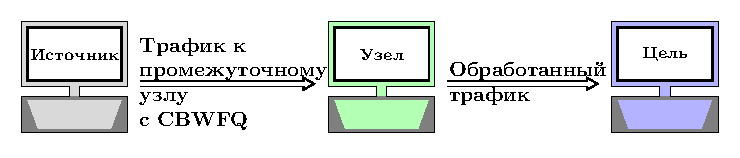
\includegraphics[scale=1.2]{pdfimages/test_scheme.pdf}
        	\caption{Схема тестовой среды.}
			\label{pic:testscheme}
        \end{figure}

		В Листинге~\ref{lst:tccmd} приведена система настройки дисциплины на промежуточном узле.

		Переменная окружения \lstinline{TESTPORT} содержит в себе номер порта,
		с которого будет отправлен трафик на сервер. При добавлении дисциплины
		на интерфейс необходимо указать пропускную способность канала; размер
		очереди по умолчанию назначается опиционально. При конфигурации класса
		во второй строке происходит назначения полосы пропускания для класса
		в процентах (возможно также назначение в bps).
        Так как CBWFQ всегда имеет класс по умолчанию, то
		при добавлении нового класса классу по умолчанию будет доставаться
		оставшаяся пропускная способность.
        В третьей строке происходит
		назначение фильтра, который будет направлять трафик с исходным портом \lstinline{TESTPORT}
		в очередь класса 1:2. На один класс можно назначит множество фильтров
		(Linux предоставляет гибкие возможности по настройке фильтрации); это не
		контролируется непосредственно дисциплиной и находится в компетенции
		пользователя. 

        \begin{figure}[ht!]
    		\center
    		\begin{lstlisting}[frame=lines,
    						  caption={Список команд для конфигурации дисциплины обслуживания CBWFQ.},
    						  label={lst:tccmd},
    						  style=tcstyle]
tc qdisc add dev eth1 cbwfq default weight 30
tc class add dev eth1 parent 1: classid 1:2 cbwfq weight 70
tc filter add dev eth1 parent 1: protocol ip u32 match ip sport $TESTPORT flowid 1:2
    		\end{lstlisting}
        \end{figure}
%$
		Для тестирования пропускной способности, которая была выделена каждому классу,
		была использована утилита iperf версии 3, которая запускалась на узле-источнике (Листинг~\ref{lst:iperfsrc}) и
		узле-цели (Листинг~\ref{lst:iperfdst}). По умолчанию iperf генерирует TCP-трафик c окном,
		указаным в командной строке на стороне сервера; с клиента на сервер передаётся трафик в два потока.

        \begin{figure}[ht!]
    		\center
    		\begin{lstlisting}[frame=lines,
    						  caption={Команда iperf на узле-источнике (клиентская сторона).},
    						  label={lst:iperfsrc}]
iperf3 -c $SERVERIP --cport $TESTPORT -P 2
    		\end{lstlisting}
        \end{figure}	
%$
        \begin{figure}[ht!]
    		\center
    		\begin{lstlisting}[frame=lines,
    						  caption={Команда iperf на узле-цели (серверная сторона).},
    						  label={lst:iperfdst}]
iperf3 -s --logfile "$EXPNUM".log
    		\end{lstlisting}
        \end{figure}
%$
%		\subsection{Сравнение с моделью WFQ в системе моделирования AnyLogic}
%
%			Для исследования корректности реализации алгоритма использовалась
%			модель CBWFQ, реализованная в системе имитационного моделирования
%			AnyLogic, которая была представлена в работе \cite{anylogic}. 
%
%			В рамках тестирования был проведён следующий эксперимент в описанной конфигурации.
%			На промежуточном и целевом узле был собран трафик с помощью утилиты \texttt{tcpdump}
%			(Листинг~\ref{lst:tcpdump}).
%
%        \begin{figure}[ht!]
%    		\center
%    		\begin{lstlisting}[frame=lines,
%    						  caption={Команда команда сбора трафика с помощью утилиты \texttt{tcpdump}.},
%    						  label={lst:tcpdump}]
%tcpdump -w $PCAPFILE -ni $INIFACE tcp and dst 10.0.4.30
%    		\end{lstlisting}
%        \end{figure}
%
%			Предполагается, что распределения интервалов между пакетами в собранном трафике на
%			целевом узле и обработанном в модели трафике, собранном на промежуточном узле должны
%			совпасть.
%			На Рисунках~\ref{pic:anylogicint1} и~\ref{pic:anylogicint2} приводятся графики,
%			вычисленные в модели AnyLogic. На них видно влияние весов на скорость
%			роста функции: функция с меньшим весом растёт быстрее.
%
%            \begin{figure}[ht!]
%            	\center
%            	\includegraphics[width=0.7\linewidth]{images/anylogicint1.png}
%            	\caption{График распределения межпакетных интервалов для класса 1 (w = 0.7) в системе AnyLogic.}
%    			\label{pic:anylogicint1}
%            \end{figure}	
%
%            \begin{figure}[ht!]
%            	\center
%            	\includegraphics[width=0.7\linewidth]{images/anylogicint2.png}
%            	\caption{График распределения межпакетных интервалов для класса 2 (w = 0.3) в системе AnyLogic.}
%    			\label{pic:anylogicint2}
%            \end{figure}	


		\subsection{Анализ точности выделения канала}

    		С использованием описанной конфигурации и команд было проведено десять экспериментов.
    		В течение экспериментов собрирались отчёты от утилиты iperf со стороны сервера в
    		течение 80-ти секунд. Отчёты представляют собой таблицу с полями:
			временной интервал (в секундах), количество переданных данных, пропускная способность
			и количество отправленных датаграмм. На каждый временной интервал таблица содержит
			описанную информацию для двух потоков.

			Результаты эксперимента можно наблюдать на Рисунке~\ref{pic:plot}.

            \begin{figure}[ht!]
            	\center
            	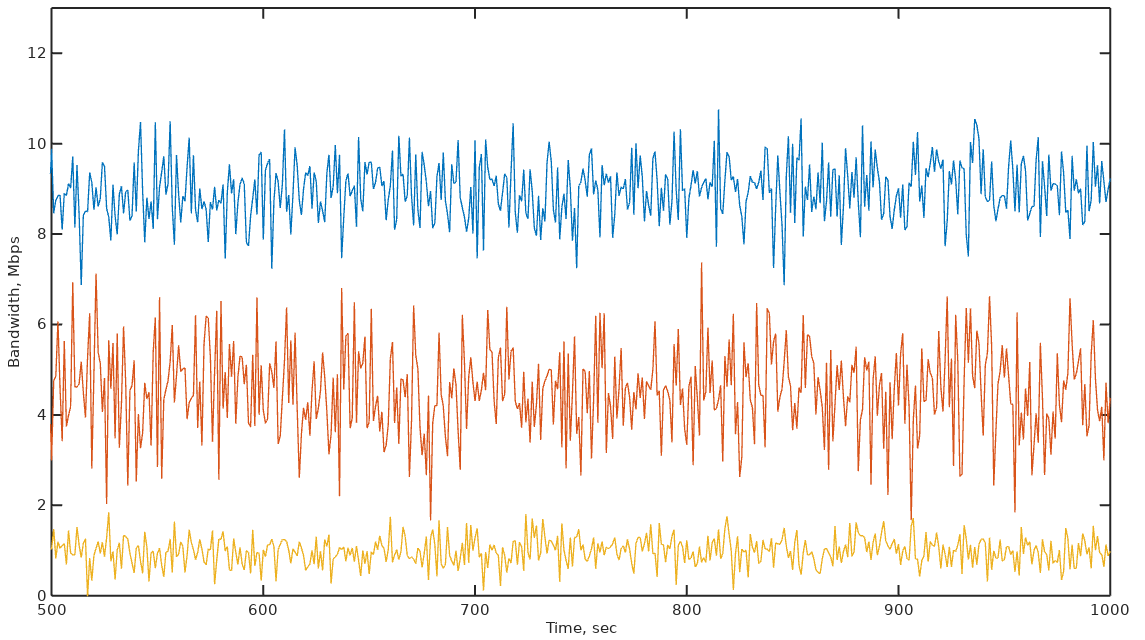
\includegraphics[width=1.1\linewidth]{pdfimages/plot.pdf}
            	\caption{График распределения доли пропускной способности (ПС) по типам трафика в течение времени.}
    			\label{pic:plot}
            \end{figure}
    %$
    		Из анализа отчётов следует, что среднее значение доли пропускной способности для первого
			класса равно $0.28 \pm 0.04$, а для второго -- $0.71 \pm 0.04$; это означает,
			что в среднем классы получают пропускную способность в соответствии с его конфигурацией.

			Далее такой экперимент проводился для разных соотношений весов первого и второго потока.
			Результаты этого эксперимента приведены в Таблице~\ref{tab:rateres}.
		
			\begin{table}[ht!]
				\center
				\begin{tabular}{|c|c|c|}
					\hline
					Весa & \mc{Доля канала\\  для класса 1} & \mc{Доля канала\\ для класса 2} \\ \hline
    				$w_1 = 0.5, w_2 = 0.5$ & $0.49 \pm 0.07$ & $0.52 \pm 0.07$\\ \hline
    				$w_1 = 0.6, w_2 = 0.4$ & $0.55 \pm 0.05$ & $0.45 \pm 0.05$\\ \hline
    				$w_1 = 0.7, w_2 = 0.3$ & $0.71 \pm 0.04$ & $0.28 \pm 0.04$\\ \hline
    				$w_1 = 0.8, w_2 = 0.2$ & $0.83 \pm 0.03$ & $0.18 \pm 0.03$\\ \hline
    				$w_1 = 0.9, w_2 = 0.1$ & $0.91 \pm 0.01$ & $0.09 \pm 0.01$\\ \hline
    				\end{tabular}
				\caption{Зависимость выделяемой доли канала для классов от указанных при концигурации весов }
				\label{tab:rateres}
			\end{table}

			Из результатов эксперимента следует, что чем больше разница между весами
			первого и второго класса, тем точнее происходит выделение канала. Это
			обуславливается тем, что при вычислении виртуального времени
			происходит целочисленные деления, из-за чего теряется точность
			для близких значениях весов.
			

